

\begin{frame}[c]\frametitle{Vidal de Battini}
    
% grafico de regiones dialectales
Separó a la Argentina en regiones dialectales
\begin{figure}
 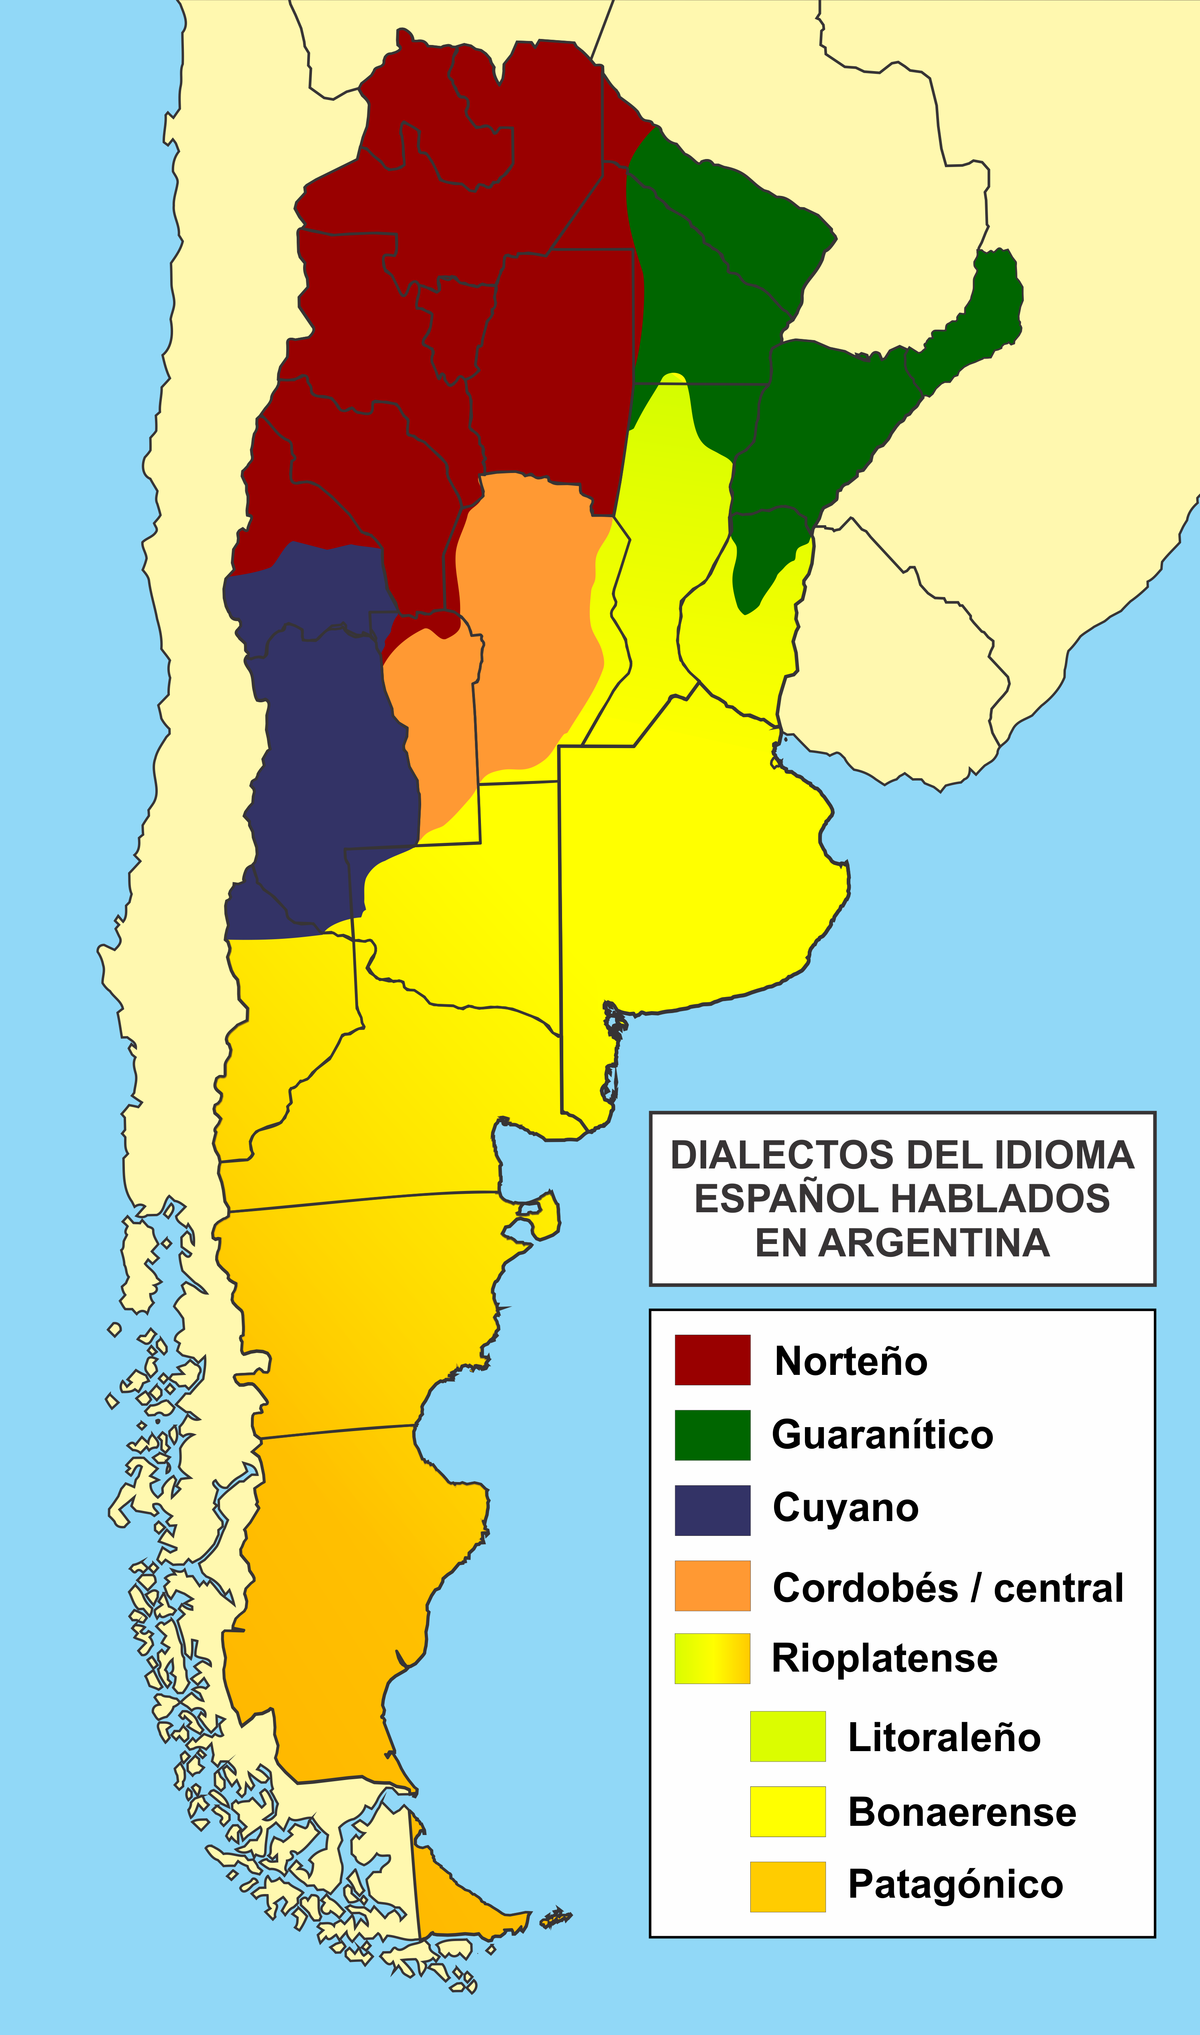
\includegraphics[height=0.7\textheight]{../src/images/presentacion/regiones_dialectales.png}
\end{figure}
\end{frame}

\begin{frame}[c]\frametitle{Método usual para detectar léxico contrastivo y las ventajas de complementar con la metodología computacional}
    
    ¿Cómo se conocían las palabras contrastivas?
    \textbf{Mediante encuestas.}
    \begin{itemize}
        \item Costosas de realizar
        \item Muy difícil de hacer de forma balanceada en distintas regiones de un país/continente.
        \item Díficil de lograr un buen cubrimiento de hablantes
        \item \alert{Se basan en el conocimiento \textit{a priori}}
    \end{itemize}
\end{frame}

% \begin{frame}[t]\frametitle{Web como un corpus}
%     % Kilgariff comentaba la riqueza de la Web para acceder a un volúmen de información, antes impensado.
%     Kilgariff: riqueza de la Web, muchos datos.
%     %Principalmente se hacían estudios estimando la frecuencia de una palabra viendo la cantidad de resultados de las consultas en un motor de búsqueda.

% \bigskip
% \begin{columns}
%     \begin{column}{0.5\textwidth}
%         \centering{\textbf{Ventajas}}
%         \begin{itemize}
%             \item Gratuito
%             \item Gran cantidad de datos
%             \item Disponible e inmediato
%         \end{itemize}
%     \end{column}
%     \begin{column}{0.5\textwidth}
%         \centering{\textbf{Utilidades}}
%         \begin{itemize}
%             \item Corrección de ortografía
%             \item Traducción de frases
%             \item Estimar el tamaño de la Web
%         \end{itemize}
%     \end{column}
% \end{columns}

% \bigskip
% \begin{block}{Cita}
% \textcquote[p. 342]{kilgarriff2003introduction}{La web es un corpus sucio, pero el uso esperado es mucho más frecuente que lo que puede considerarse como ruido.} 
% \end{block}

% \end{frame}